\subsection{De drempelspanning van de ISFET uitlezen} \label{sec:ISFETLees}

De pH sensor is het onderdeel van het systeem die de pH waarde van de te meten oplossing uitleest. Dit onderdeel zit voor de versterker, zoals uitgebeeld in \cref{fig:pHInSchema}.
\begin{figure}[!htbp]
    \centering
    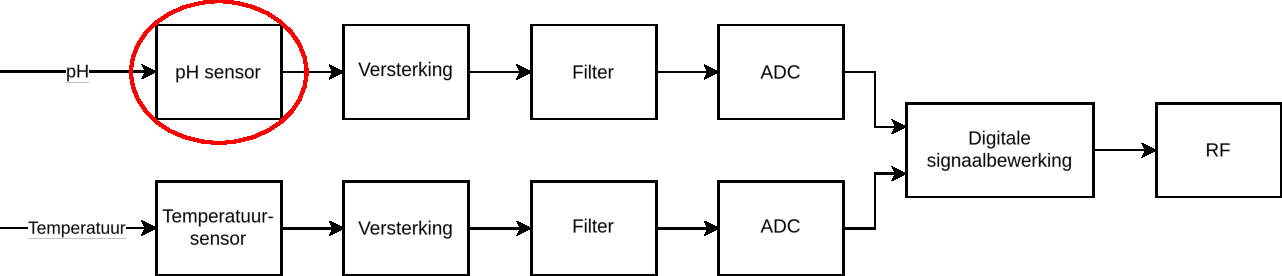
\includegraphics[width=0.95\textwidth]{signaalblokjes/pHInSchema.pdf}
    \caption{Het onderdeel van \cref{fig:analogeBewerkingsFunctie} waar dit hoofdstuk over gaat.}
    \label{fig:pHInSchema}
\end{figure}

% TODO: Bronnen
Om de pH waarde van de ISFET uit te lezen moet de drempelspanning gemeten worden. Deze is namelijk linear afhankelijk van de pH waarde \cite{iontjes}.
Om de drempelspanning te meten kan een regelsysteem gebruikt worden. Door de gate-source spanning te variëren kunnen $U_{ds}$ en $I_{ds}$ van de ISFET constant gehouden worden.

Er zijn meerdere mogelijke implementaties van een dergelijk regelsysteem. Twee hiervan zijn afgebeeld in \cref{fig:measureCircuits}.
Elk van deze schakelingen gebruikt een nullor om de drain-source spanning van de ISFET gelijk te houden. Ook gebruikt elk van deze schakelingen een referentiespanning. De implementatie van deze referentiespanning wordt verder besproken in \cref{sec:referenceVoltage}.

De drain-source spanning $U_{ds}$ en drain-source stroom $I_{ds}$ zijn van te voren gedefinieerd. Deze zijn te vinden in de datasheet van de ISFET \cite{isfet}. Uit deze twee waardes kunnen de referentiespanningen en weerstandswaardes van de schakelingen gevonden worden.
Voor de schakeling in \cref{fig:measureCurrent} is de spanningsreferentie te vinden door middel van \cref{eq:URefSource}.
\begin{equation}\label{eq:URefSource}
    U_{ref,s} = U_{dd} - U_{ds}
    \tagaddtext{[\si{\volt}]}
\end{equation}
Voor \cref{fig:measureResistor} is de referentiespanning gelijk aan de drain-source spanning, te zien in \cref{eq:URefDrain}.
\begin{equation}\label{eq:URefDrain}
    U_{ref,d} = U_{ds}
    \tagaddtext{[\si{\volt}]}
\end{equation}
Voor de waarde van de weerstand in \cref{fig:measureResistor} kan \cref{eq:measureResistorVal} gebruikt worden.
\begin{equation}\label{eq:measureResistorVal}
    R = \frac{U_{dd} - U_{ds}}{I_{ds}}
    \tagaddtext{[\si{\ohm}]}
\end{equation}


\begin{figure}[!htbp]
    \centering
    \begin{subfigure}[b]{0.45\textwidth}
        \centering
        \def\svgwidth{\textwidth}
        \input{img/ISFETCircuitBest.pdf_tex}
        \caption{Met een weerstand aan de drain.}
        \label{fig:measureResistor}
    \end{subfigure}
    \hfill
    \begin{subfigure}[b]{0.45\textwidth}
        \centering
        \def\svgwidth{\textwidth}
        \input{img/ISFETCircuit.pdf_tex}
        \caption{Met een stroombron aan de source.}
        \label{fig:measureCurrent}
    \end{subfigure}
    \caption{De uitleesschakelingen voor de ISFET.}
    \label{fig:measureCircuits}
\end{figure}

Beide schakelingen hebben voor- en nadelen.
Bij de schakeling in \cref{fig:measureResistor} zit de source van de ISFET direct verbonden met de ground. Dit heeft als voordeel dat de uitgang van de nullor gelijk is aan de gate-source spanning. Hierdoor hoeft de nullor lagere spanningen te genereren om de gate-source spanning van de ISFET naar de goede waarde te krijgen. De spanning die de nullor moet genereren in het geval van een drain weerstand is te vinden door middel van \cref{eq:nullorVoltageDrain}. In het geval van een stroombron aan de source is dat \cref{eq:nullorVoltageSource}.

\begin{equation}\label{eq:nullorVoltageDrain}
    U_{nullor,d} = U_{gs}
    \tagaddtext{[\si{\volt}]}
\end{equation}
\begin{equation}\label{eq:nullorVoltageSource}
    U_{nullor,s} = U_{gs} + U_{ref,s}
    \tagaddtext{[\si{\volt}]}
\end{equation}

De schakeling met een stroombron aan de source heeft de mogelijkheid om betere ruiseigenschappen te hebben. De stroombron kan ook een hogere impedantie hebben dan de weerstand. Het vermogensverbruik van de schakeling in \cref{fig:measureResistor} is echter duidelijk minder, dus is dit de schakeling die gebruikt zal worden.

\subsubsection{Ruis}

De meetschakeling heeft een aantal ruisbronnen. De nullor heeft een ingangsstroom- en spanninsruisbron. Daarnaast genereert de weerstand ook thermische ruis. Deze ruisbronnen zijn te zien in \cref{fig:measureNoise}.
\begin{figure}[!htbp]
    \centering
    \def\svgwidth{0.6\textwidth}
    \input{img/ISFETCircuitBestNoise.pdf_tex}
    \caption{De ruisbronnen van de meetschakeling.}
    \label{fig:measureNoise}
\end{figure}


Omdat $U_{ds}$ en $I_{ds}$ van de ISFET niet veranderen, kan de impedantie ervan gezien worden als weerstand, met een waarde van $\frac{U_{ds}}{I_{ds}}$. Hierdoor wordt er een nieuwe ruisbron $i_{n,ds}$ toegevoegd. Met deze weerstand kunnen de bronnen $i_{n,ref}$, $i_{n,R}$ en $i_{n,ds}$ worden getransformeerd naar een spanningsbron $u_{n,in}$ aan de ingang van de nullor.
Vervolgens kan deze, samen met de spanningsruisbronnen $u_{n,ref}$ en $u_{n,n}$ naar de uitgang getransformeerd worden. Dit komt uit op een enkele spanningsruisbron aan de uitgang, zoals te zien is in \cref{fig:measureNoiseMoved}. De spectrale spanningsruisdichtheid van deze ruisbron is te berekenen door middel van \cref{eq:measureNoiseOut}.

\begin{equation}\label{eq:measureNoiseOut}
    S_{u_{{n,out}}} = \left(S_{u_{{n,ref}}} + S_{u_{{n,n}}} + S_{i_{n,in}}\left(Z_{fet} // R\right)^2\right) \cdot H^2(\ph)
    \tagaddtext{[\si{\volt\squared\per\hertz}]}
\end{equation}
\begin{equation}
    S_{i_{{n,in}}} = S_{i_{{n,n}}} + S_{i_{{n,R}}} + S_{i_{{n,ds}}}
    \tagaddtext{[\si{\ampere\squared\per\hertz}]}
    \label{eq:measureNoiseCurrentIn}
\end{equation}


De definities van deze ruisbronnen zijn te vinden in \cref{tab:measureNoiseValues}.

\begin{table}[!htbp]
    \centering
    \begin{tabular}{c|l}
        Ruisbron & Waarde \\
        \hline
        $S_{u_{{n,ref}}}$ & Zie \cref{sec:referenceVoltage} \\
        $S_{u_{{n,n}}}$   & Implementatie nullor \\
        $S_{i_{{n,n}}}$   & Implementatie nullor \\
        $S_{i_{n,in}}$    & \Cref{eq:measureNoiseCurrentIn} \\
        $S_{i_{{n,R}}}$   & $\frac{4kT}{R}$ \\
        $S_{i_{{n,ds}}}$  & $4kT\frac{I_{ds}}{U_{ds}}$ \\
    \end{tabular}
    \caption{Waar de waardes van de ruisbronnen vandaan gehaald kunnen worden.}
    \label{tab:measureNoiseValues}
\end{table}

\begin{figure}[!htbp]
    \centering
    \def\svgwidth{0.6\textwidth}
    \input{img/ISFETCircuitBestNoiseMoved.pdf_tex}
    \caption{De meetschakeling met verschoven ruisbronnen.}
    \label{fig:measureNoiseMoved}
\end{figure}

De overdracht van deze schakeling is gelijk aan de uitgangsspanning gedeeld door de ingangsspanning van de nullor. Door de werking van de schakeling blijft de ingansspanning altijd gelijk en is de uitgangsspanning lineair afhankelijk van de pH waarde. Hierdoor is de overdracht $H(\ph)$ een functie van de gemeten pH waarde.

Deze overdrachtsfunctie is gedefinieerd in \cref{eq:measureTransfer}, en is een functie van de uitgangsspanning. De uitgangsspanning is een functie van de pH waarde, en is te vinden in \cref{eq:measureOutVoltage}. Hierin is $C_{pH}$ de gevoeligheid van de sensor, die gegeven wordt in $\si{\milli\volt\per\ph}$, en is $U_7$ de uitgangsspanning op pH 7.

\begin{equation}
    H(\ph) = \frac{U_o(\ph)}{U_{ref}}
    \label{eq:measureTransfer}
\end{equation}

\begin{equation}\label{eq:measureOutVoltage}
    U_o(\ph) = C_{pH}\ph + U_7
    \tagaddtext{[\si{\volt}]}
\end{equation}
Door de hoogste uitgangsspanning $U_{o,max}$ te nemen, kan de maximale uitgangsruis berekend worden. Deze is te vinden in \cref{eq:measureNoiseFull}.

\begin{equation}\label{eq:measureNoiseFull}
    S_{u_{{n,out}}} = \left(S_{u_{{n,ref}}} + S_{u_{{n,n}}} + S_{i_{{n,in}}}\left(Z_{fet} // R\right)^2\right) \cdot \left(\frac{U_{o,max}}{U_{ref}}\right)^2
    \tagaddtext{[\si{\volt\squared\per\hertz}]}
\end{equation}

Aangezien er geen frequentieafhankelijkheden voorkomen kan de uitgangsspanningsruis uitgerekend worden door de spectrale ruisdichtheid te vermenigvuldigen met de bandbreedte. Dit wordt gedaan in \cref{eq:measureNoiseVoltage}.
\begin{equation}\label{eq:measureNoiseVoltage}
    u_{n,out} = \sqrt{B \cdot S_{u_{{n,out}}}}
    \tagaddtext{[\si{\volt}]}
\end{equation}

\subsubsection{Vermogen}
Het vermogensverbruik van deze schakeling is gedefinieerd in \cref{eq:measurePower}, waar $P_n$ het vermogensverbruik van de nullor implementatie is.
\begin{equation}\label{eq:measurePower}
    P = P_n + U_{dd}I_{ds}
\end{equation}


% \subsubsection{Versterker}
% Aangezien de uitgang van de ISFET een meetbare spanning produceert (\qty{1.8}{\volt} tot \qty{2.2}{\volt} volgens \cite{isfet}) zal er geen versterker nodig zijn om de pH waarde te kunnen meten. Wel zou een level-shifter gebruikt kunnen worden in combinatie met een versterker om zo het volledige bereik van de ADC te gebruiken. Dit voegt echter meer ruis en complexiteit toe aan het systeem, waardoor er in deze iteratie voor is gekozen om dit niet te doen.
%TODO: dit^^